\documentclass[11pt]{article}
\usepackage[margin=1in]{geometry}
\usepackage{amsmath,amssymb}
\usepackage{graphicx}
\usepackage{booktabs}
\usepackage{float}

\begin{document}

%======================================================================
\section{Does contrastive decoding act where the hallucination is decided?}
%======================================================================

\paragraph{Context.}
Contrastive decoding (CD) subtracts a degraded amateur branch from the expert to
push the model away from hallucinated answers. If this works as intended, then at
the token where the model commits to an answer the subtraction should be
\emph{selective}: it should lower the score of answers that are actually
hallucinations while leaving correct answers unchanged. A shift that moves every
answer by the same amount, regardless of whether it is a hallucination, is not a
correction but a uniform translation of the decision. We test which of the two it
is by looking inside the model, at the representation it uses to decide.

\paragraph{Methodology.}
We restrict the test to the questions the model answers ``Yes,'' the only answers on
which a hallucination can occur, and split them into hallucinations $\mathcal{H}$
(object absent, model says Yes) and correct calls $\mathcal{T}$ (object present,
model says Yes). To read a decision off a layer we use the model's own head (the
logit lens): apply the final RMSNorm and unembedding to the layer's hidden state,
restrict to the ``Yes''/``No'' tokens, and take the margin
$m_\ell=\max_{\text{Yes}}z_\ell-\max_{\text{No}}z_\ell$, positive when the model would
answer ``Yes.'' Running this on the clean (expert) and noised (amateur) passes gives
$m^{E}_\ell,m^{A}_\ell$; since CD forms $(1+\alpha)z^{E}-\alpha z^{A}$ and the margin
is linear in the logits,
\begin{equation}
m^{CD}_\ell = m^{E}_\ell + \alpha\,\Delta_\ell,\qquad \Delta_\ell = m^{E}_\ell - m^{A}_\ell,
\end{equation}
so $\Delta_\ell$ is one number per sample per layer: the log-odds CD adds to the
decision, negative when it suppresses ``Yes'' (the correcting direction on a
hallucination) and positive when it reinforces it. We also fit a linear probe
(logistic regression, standardized features, 5-fold CV, out-of-fold probabilities)
on the hidden state at each layer and report its AUC.

\emph{Experiment~1 (direct test).} Layer-wise analysis is the natural lens here
because the final answer is nothing more than a readout of a hidden state: the
decision is formed inside the stack, at whatever depth the hallucination signal
becomes linearly present, and only then projected to the ``Yes''/``No'' tokens. If CD
genuinely corrected the hallucination, it would have to engage \emph{that}
representation, so its effect should be largest at, or at least track, the layer where
the hallucination is decided. A correction that lands where the deciding information
is not yet present, or that ignores that depth entirely, is acting on something other
than the mechanism that produced the error. The intuitive test is therefore to ask
where, across depth, the hallucination is decided and whether that is where CD acts.
We plot, per layer, how decodable the hallucination is (a probe over the absent
samples predicting the false ``Yes'') against CD's mean effect $\overline{\Delta}_\ell$
on $\mathcal{H}$ (Figure~\ref{fig:direct}). This is the natural first cut, but two problems keep it
from settling the question. First, the residual stream is additive: a shift written
at any layer propagates to the output, so a mismatch between where the hallucination
is decoded and where $\overline{\Delta}_\ell$ peaks does not by itself prove CD acts
in the wrong place. Second, $\overline{\Delta}_\ell$ is a magnitude and a group mean;
a large average shift says nothing about whether CD \emph{distinguishes} hallucinated
from correct answers, which is what a correction must do.

\emph{Experiment~2 (selectivity).} To remove both problems we test, at every layer,
whether $\Delta_\ell$ carries hallucination-specific information rather than where it
is largest. Since $\mathcal{H}$ is absent and $\mathcal{T}$ present, telling them
apart is exactly object presence, so the probe of presence (Probe~A) is the matched
baseline for what CD would need. We compute four layer-wise quantities on
$\mathcal{H}\cup\mathcal{T}$ (Figure~\ref{fig:battery}): (i) a \emph{selectivity}
AUC, whether $-\Delta_\ell$ ranks $\mathcal{H}$ above $\mathcal{T}$ for suppression
($0.5$ if blind); (ii) whether the amateur branch even forms the presence signal,
the AUC of $m^{A}_\ell$ vs.\ the clean $m^{E}_\ell$; (iii) the fraction of
$\mathcal{H}$ with $\Delta_\ell>0$; and (iv) $R^2_\ell$, the share of the variance of
$\Delta_\ell$ explained by hallucination status. Because these are layer-resolved and
about information content, a null result at \emph{every} depth closes the additivity
loophole: there is no layer, early or late, at which a selective correction could
hide.

\paragraph{Experimental details.}
We run POPE--COCO ($9000$ questions) on LLaVA-1.5-7B. For each question we take two
single forward passes at $T=1$, a clean pass and a noised pass corrupted by the
method's own $\mathrm{add\_diffusion\_noise}(\cdot,900)$, and store the logit-lens
Yes/No margins at the final prompt-token position for all $33$ layers. Of the $3710$
questions answered ``Yes,'' $|\mathcal{H}|=257$ are hallucinations and
$|\mathcal{T}|=3453$ correct positives. Probe~A is fit on all samples; the
hallucination-decodability probe of Experiment~1 (Probe~B) on the absent samples.
Extraction ran on a single NVIDIA L4; the probes and analyses are offline on CPU. We
use $\alpha=1$, and verified the lens reproduces the true final logits to a mean
absolute error of $1.7\times10^{-3}$ log-odds.

\paragraph{Results.}
Experiment~1 (Figure~\ref{fig:direct}) shows the hallucination is decodable from
layer $12$ (probe AUC $\to 1.0$), while CD's effect is near zero until then, peaks at
layer $19$ ($\overline{\Delta}=+17.9$), and decays to $+3.32$ at the readout. Two
features stand out: CD's effect is offset several layers past where the hallucination
is settled, and it is \emph{positive} at every layer, i.e.\ it reinforces the false
``Yes'' rather than suppressing it. On its own, though, this is only suggestive: by
the additivity argument the depth offset need not imply CD acts in the wrong place,
and a positive mean does not establish that CD treats hallucinated and correct
answers alike.

Experiment~2 (Figure~\ref{fig:battery}, Table~\ref{tab:nums}) settles both. Object
presence is decodable from layer $8$ (Probe~A AUC crosses $0.95$, rising to $0.99$;
even the $1$-D margin separates $\mathcal{H}$ from $\mathcal{T}$ at AUC $0.86$), so
the information a selective CD needs is present. Yet CD's selectivity never leaves
$[0.40,0.60]$ at any depth and is $0.52$ at the readout; its shift reinforces the
false ``Yes'' for $96.5\%$ of hallucinations at the readout, with the fraction pushed
toward ``Yes'' locking near $0.95$ from layer $17$; and hallucination status explains
at most $0.7\%$ of the variance of $\Delta_\ell$ anywhere, including layer $19$ where
the raw shift is largest. The amateur branch keeps a weaker but real presence signal
(AUC $0.78$ vs.\ the clean $0.94$), so CD is not blind for lack of a signal; it simply
does not encode presence at any depth. Because the selectivity is null at every
layer, the additivity loophole is closed. Two limits remain: this is the single
forced yes/no token, not free-form generation, and it isolates the contrastive term
$m^{E}+\alpha\Delta$ (the decoder also applies a plausibility mask); changing $\alpha$
scales $\Delta$ but cannot flip its sign, so no $\alpha$ recovers suppression once
$\Delta>0$ for $96.5\%$ of cases.

\paragraph{What we infer.}
From layer $8$ the model carries a clean linear representation of object presence,
exactly what separates a hallucinated ``Yes'' from a correct one, but CD's shift never
uses it: its selectivity sits at chance, it explains under $1\%$ of the shift's
variance, and where it acts most strongly it pushes hallucinations further toward
``Yes.'' Contrastive decoding therefore does not correct hallucinations at the point
of decision; it applies a uniform, one-sided translation of the Yes-vs-No margin,
blind to whether an answer is a hallucination, so any measured reduction is a
threshold effect rather than a correction of the mechanism that produces it.

\begin{figure}[H]
  \centering
  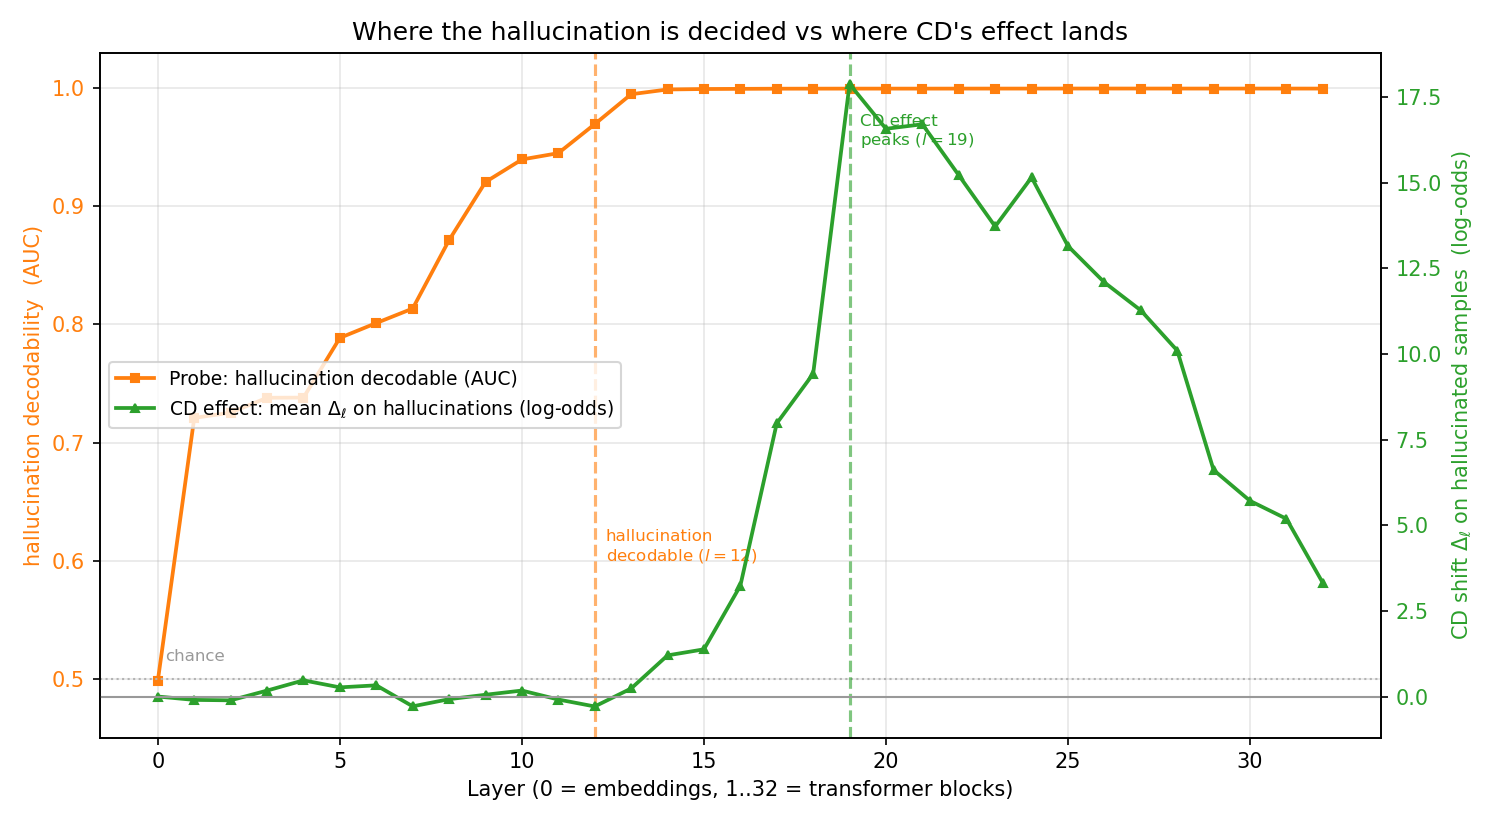
\includegraphics[width=0.86\linewidth]{halluc_auc_vs_cd_effect.png}
  \caption{Experiment~1 (direct test). Hallucination decodability (orange, left) is
  complete by layer $12$, while CD's mean effect $\overline{\Delta}_\ell$ on
  $\mathcal{H}$ (green, right, log-odds) is near zero until then, peaks at layer $19$,
  and stays positive throughout, i.e.\ CD reinforces the false ``Yes.'' Suggestive but
  not conclusive: additivity means the depth offset is not decisive, and a group-mean
  magnitude does not establish selectivity.}
  \label{fig:direct}
\end{figure}

\begin{figure}[H]
  \centering
  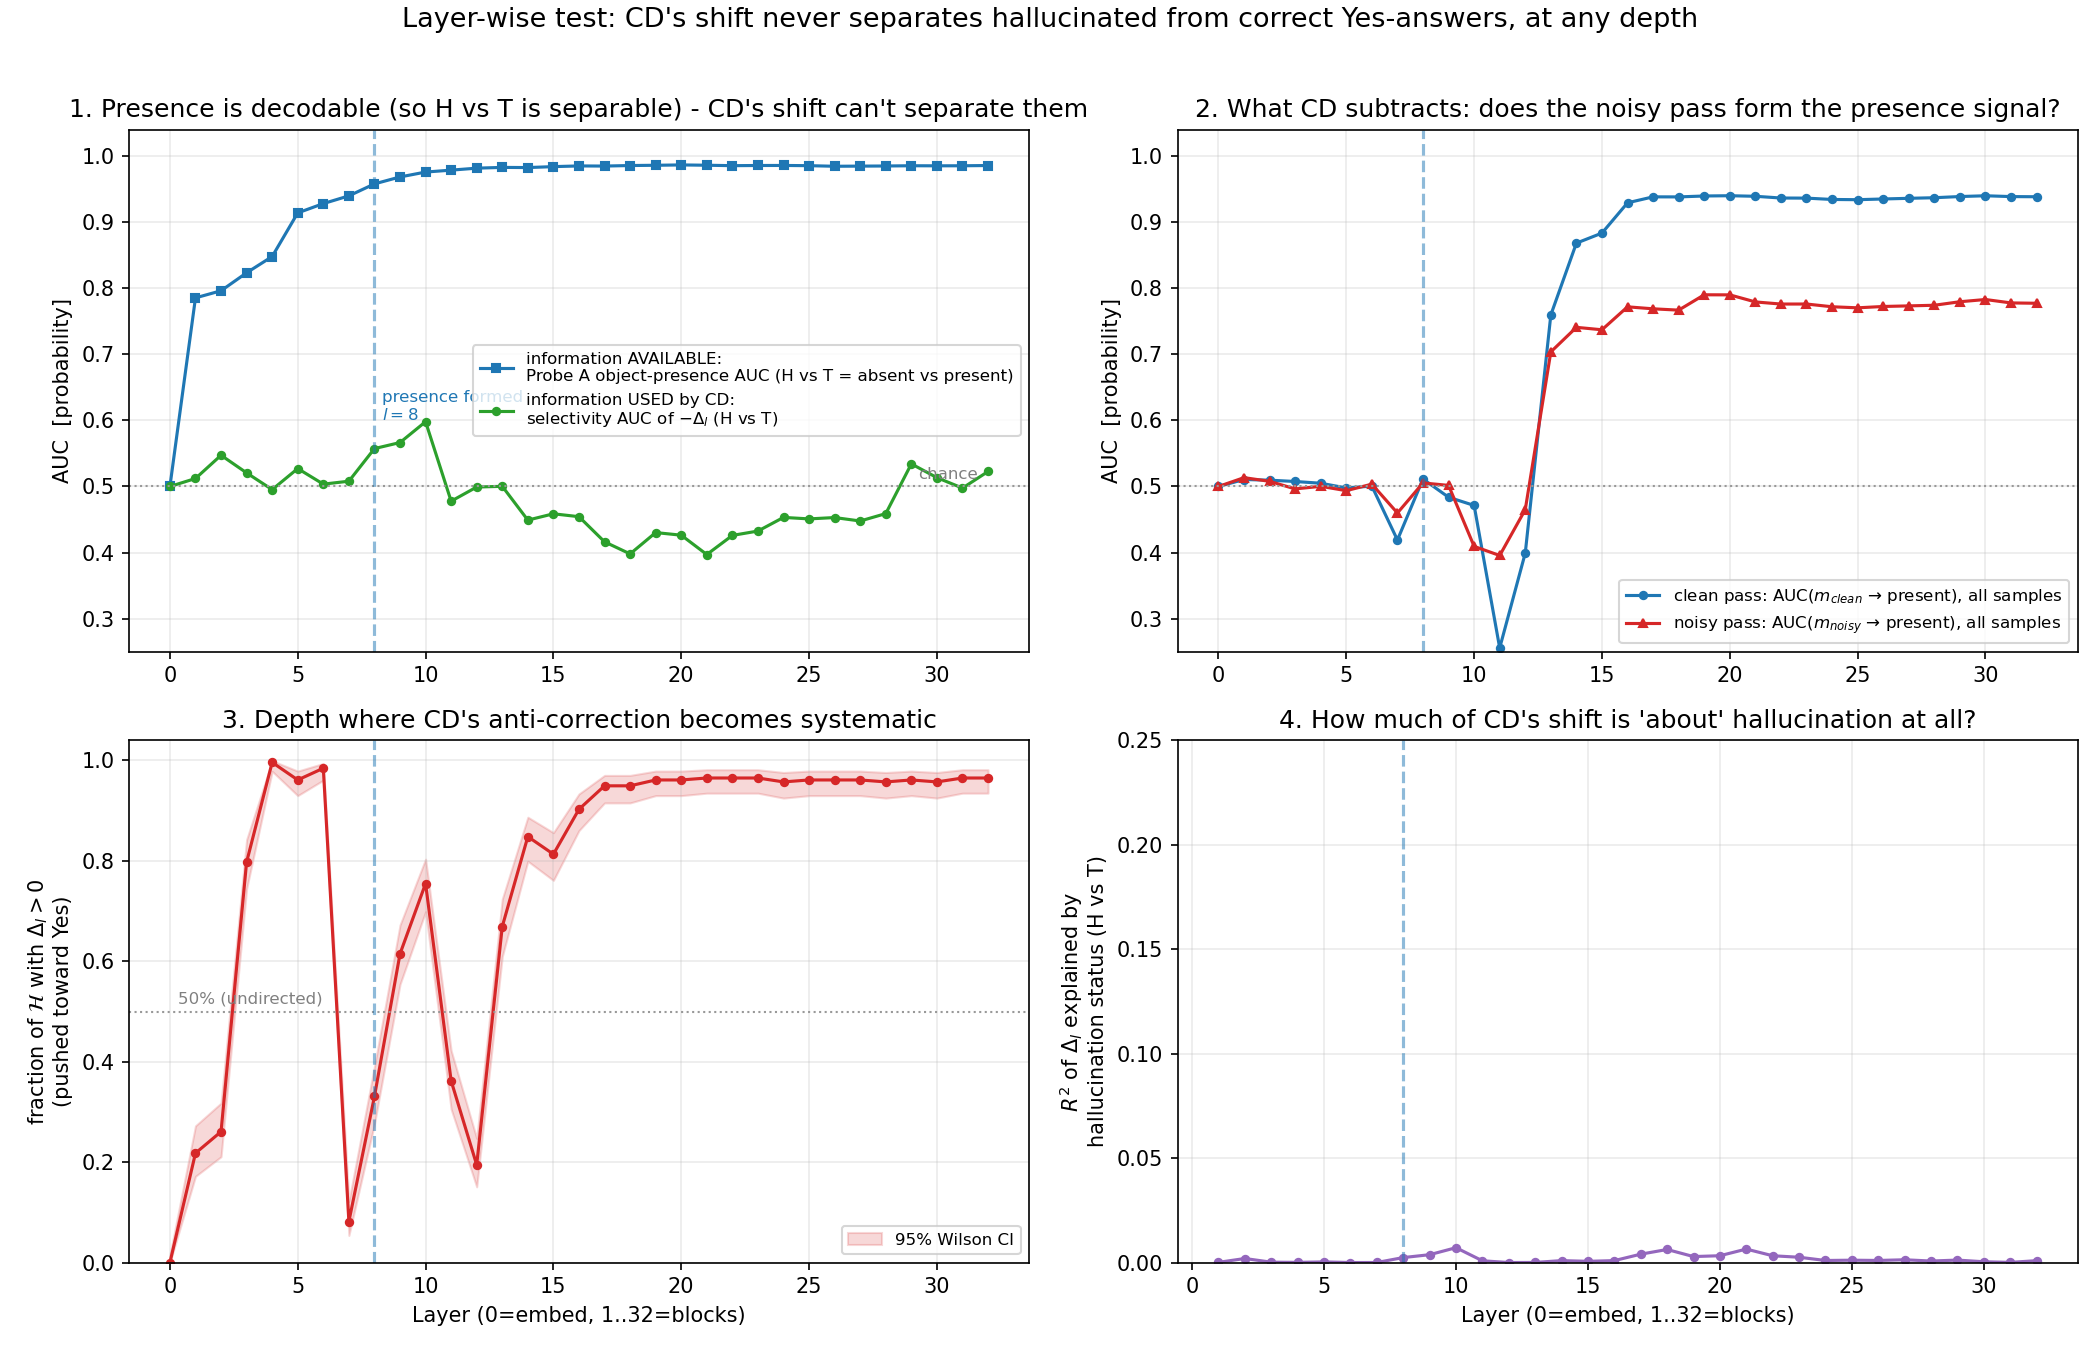
\includegraphics[width=\linewidth]{layerwise_battery.png}
  \caption{Experiment~2 (selectivity). (1) Presence (the $\mathcal{H}$-vs-$\mathcal{T}$
  distinction) is decodable from layer $8$ (Probe~A, blue), yet CD's selectivity
  (green) stays at chance. (2) The amateur branch's presence signal is degraded (AUC
  $0.78$ vs.\ $0.94$) but not absent. (3) The fraction of $\mathcal{H}$ pushed toward
  ``Yes'' locks near $0.95$ from layer $17$ ($95\%$ Wilson interval). (4) Hallucination
  status explains under $1\%$ of the variance of $\Delta_\ell$ at all depths.}
  \label{fig:battery}
\end{figure}

\begin{table}[H]
  \centering
  \begin{tabular}{lc}
    \toprule
    Quantity & Value \\
    \midrule
    Answered ``Yes'': hallucinated $\mathcal{H}$ / correct $\mathcal{T}$ & $257\,/\,3453$ \\
    Presence decodable (Probe~A AUC $\ge 0.95$) from layer & $8$ \\
    Presence AUC: Probe~A / in-population margin & $0.99\,/\,0.86$ \\
    Selectivity AUC of $-\Delta_\ell$: range / readout & $[0.40,\,0.60]\,/\,0.52$ \\
    Presence AUC at readout: clean / noisy branch & $0.94\,/\,0.78$ \\
    Fraction of $\mathcal{H}$ with $\Delta>0$ at readout & $0.965$ \\
    Variance explained $R^2_\ell$: max / readout & $0.007\,/\,0.0009$ \\
    Mean shift $\overline{\Delta}$ at readout: $\mathcal{H}$ / all & $+3.32\,/\,+1.23$ \\
    \bottomrule
  \end{tabular}
  \caption{Numerical results ($\alpha=1$), from the per-sample logit-lens margins over
  all $9000$ questions.}
  \label{tab:nums}
\end{table}

\end{document}
